\newcommand{\anonsection}[1]{\section*{#1}\addcontentsline{toc}{section}{#1}}
\newcommand{\anonsubsection}[1]{\subsection*{#1}\addcontentsline{toc}{subsection}{#1}}
\newcommand{\anonsubsubsection}[1]{\subsubsection*{#1}\addcontentsline{toc}{subsubsection}{#1}}
\documentclass[11pt]{article}
\usepackage{a4wide}
\usepackage[utf8]{inputenc}
\usepackage[russian]{babel}
\usepackage{graphicx}
\usepackage{amsmath}
\usepackage{amsfonts}
\usepackage{caption}
\usepackage{subfig}
\usepackage[left=3cm,right=3cm, top=3cm,bottom=3cm,bindingoffset=0cm]{geometry}
\usepackage{hyperref}

\newtheorem{theorem}{Теорема}
\newtheorem{definition}{Определение}
\newtheorem{notion}{Замечание}

\begin{document}

\thispagestyle{empty}

\begin{center}
\ \vspace{-3cm}


\includegraphics[width=0.5\textwidth]{msu.png}\\
{\scshape Московский государственный университет имени М.~В.~Ломоносова}\\
Факультет вычислительной математики и кибернетики\\
Кафедра системного анализа

\vfill

{\LARGE Отчет о практическом задании по курсу ``Оптимальное управление'' }

\vspace{1cm}

{\Huge\bfseries <<Построение множества достижимости>>}
\end{center}

\vspace{1cm}

\begin{flushright}
  \large
  \textit{Студент 315 группы}\\
  Е.\,В.~Гуров

  \vspace{5mm}

  \textit{Руководитель практикума}\\
  к.ф.-м.н., доцент П.\,А.~Точилин
\end{flushright}

\vfill

\begin{center}
Москва, 2021
\end{center}
\newpage

\tableofcontents
\newpage

\anonsection{Постановка задачи}
 Задано обыкновенное дифференциально уравнение:
\[ \ddot{x} + \dot{x} + 5x^5 + x \sin(x^3) = u, \]
где \( x \in \mathbb{R}, u \in \mathbb{R} \). На возможные значения управляющего параметра \( u \) наложено ограничение: \( u \in [-\alpha, \alpha] \). Задан начальный момент времени \( t_0 = 0 \) и начальная позиция \( x(t_0) = \dot{x}(t_0) \). Необходимо построить множество достижимости \( X(t, t_0,   x(t_0), \dot{x}(t_0)) \)(множество пар (x(t), \( \dot{x}(t) \))) в классе программных управлений в заданный момент времени \( t \ge t_0 \).
\begin{enumerate}
	\item Необходимо написать в среде Matlab функцию \textbf{reachset(alpha, t)}, которая по заданным параметрам \( \alpha > 0, t \ge t_0 \) рассчитывает приближенно множество достижимости \( X(t, t_0, x(t_0), \dot{x}(t_0)) \). На выходе функции --- два массива \( X, Y \) с упорядоченными координатами точек многоугольника, образующего границу искомого множества. Точки в этих массивах должны быть упорядочены так, чтобы результаты работы функции без дополнительной обработки можно было подавать на вход функциям визуализации(например, \textbf{plot}). Предусмотреть такой режим работы функции, при котором она возвращает также координаты линий переключения оптимального управления(с возможностью их визуализации).
	\item Необходимо реализовать функцию \textbf{reachsetdyn(alpha, t1, t2, N, filename)}, которая, используя функцию \textbf{reachset(alpha, t)}, строит множества достижимости жля моментов времени \( \tau_i = t_1 + \frac{(t2-t1)i}{N} \ , \ i = 0,1,\dots,N\). Здесь \( t_2 \ge t_1 \ge t_0, \ N \) --- натуральное число. Для каждого момента времени \( \tau_i \) функция должна отобразить многоугольник, аппроксимирующий границу множества достижимости. Результат работы функции должен быть сохранен в виде видео-файла \textbf{filename.avi}. Необходимо также предусмотреть вариант работы функции(при отсутствии параметра \textbf{filename}) без сохранения в файл, с выводом непосредственно на экран. Как частный случай, функция должна иметь возможность строить границу множества достижимости в один фиксированный момент времени(при \( t_2 = t_1). \)
	\item В соотвествующем заданию отчете необходимо привести все теоретические выклдаки, сделанные в ходе построения множества достижимости, описать схему алгоритма построения множества достижимости программой, привести примеры построенных множеств достижимости(с иллюстрациями), исследовать зависимость множества достижимости от величины параметра \( \alpha \). Все вспомогательные утверждения(за исключением принципа максимума Понтрягина), указанные в отчете, должны быть доказаны.
\end{enumerate}
\newpage
\anonsection{Теоретические выкладки}
Начнем анализ задачи с определения множества достижимости.
\begin{definition}
	Множеством достижимости \( X (t,t_0,x_0) \) называют множество всех точек \( x \in \mathbb{R}^n \), таких, что существует допустимое управление \(u \), переводящее систему за время \( t - t_0 \) из положения \( x_0 \) в положение \( x \), или иначе:
	\[ X(t,t_0,x_0) = \left\{ x \in \mathbb{R}^n \middle| \exists u \in \mathcal{U} : x(t,t_0,x_0,u(\cdot)) = x \right\}, \]
	где \( \mathcal{U} \) --- класс допустимых управлений.
\end{definition}
\begin{theorem}[Принцип максимума Понтрягина]
Пусть дана система в \( \mathbb{R}^n \):
\[ \dot{x} = f(x,u), \]
где \( f(x,u) \) и \( \frac{\partial f}{\partial x}(x, u) \) --- непрерывные функции.Пусть \( \mathcal{U} \) --- множество допустимых управлений на отрезке \( 0 \le t \le T \). Пусть некоторому допустимому управлению \( u^*(\cdot) \) соответствует решение \( x^*(\cdot) \) с концом \( x^*(T) \), лежащим на границе множества достижимости \( X[T] \). Тогда существует нетривиальная сопряженная вектор-функция \( \psi^*(t) \), удовлетворяющая системе уравнений:
\[ \dot{\psi} = - \langle \psi, \frac{\partial f}{\partial x}(x^*(t), u^*(t))\rangle, \]
такая, что принцип максимума \( \mathcal{H}(\psi^*(t), x^*(t), u^*(t)) = \mathcal{M}(\psi^*(t), x^*(t)) \) выполняется почти всюду по \( t \). Если при этом управление ограничено, то функция \( \mathcal{M}(\psi^*(t), x^*(t)) \) почти всюду постоянна. Здесь \( \mathcal{H} \) --- функция Гамильтона-Понтрягина, имеющая вид:
\[ \mathcal{H}(\psi, x, u) = \langle \psi, f(x,u) \rangle = \psi_1 f_1 (x, u) + \dots + \psi_n f_n(x,u), \]
а функция \( \mathcal{M} \):
\[ \mathcal{M}(\psi^*(t), x^*(t)) = \max\limits_{u \in \mathcal{U}}\mathcal{H}(\psi, x, u). \]
\end{theorem}
Запишем дифференциальное уравнение из условия задачи в виде системы. Для этого сделаем замену \( x_1 = x , x_2 = \dot{x} \). Получим: 
\begin{equation}\label{dif_syst}
	\begin{cases}
		\dot{x}_1 = x_2,
		\\
		\dot{x}_2 = u - x_2 - 5 x_1^5 - x_1 \sin(x_1^3),
		\\
		x_1(t_0) = 0,
		\\
		x_2(t_0) = 0.
	\end{cases}
\end{equation}
Функция Гамильтона-Понтрягина в таком случае будет выглядеть так:
\begin{equation}\label{HP_function}
	\mathcal{H} = \psi_1 x_2 + \psi_2(u - x_2 - 5 x_1^5 - x_1 \sin(x_1^3)).
\end{equation}
Сопряженная система:
\begin{equation}\label{conj_syst}
	\begin{cases}
		\dot{\psi}_1(t) = -\frac{\partial \mathcal{H}}{\partial x_1} = \psi_2(25x_1^4 + \sin(x_1^3) + 3x_1^3\cos(x_1^3)),
		\\
		\dot{\psi}_2(t) = -\frac{\partial \mathcal{H}}{\partial x_2} = -\psi_1 + \psi_2.
	\end{cases}
\end{equation}
Из (\ref{HP_function}) видно, что оптимальное уравление выражается следующим образом:
\begin{equation}\label{opt_control}
	u^*(t) = \begin{cases}
				\alpha, & \psi_2 > 0,
				\\
				[-\alpha; \alpha], & \psi_2 = 0,
				\\
				-\alpha, & \psi_2 < 0.	
		      \end{cases}
\end{equation}
Отметим, что особый режим невозможен, так как если \( \psi_2(t) \equiv 0\ , \ \forall t \in (t_1; t_2) \), то из (\ref{conj_syst}) следует, что \( \psi_1 \equiv 0 , \ , \forall t \in (t_1; t_2) \), что противоречит условию нетривиальности \( \psi \).
\begin{theorem}
	Пусть дана система:
	\[ \begin{cases}
		\dot{x}_1 = x_2,
		\\
		\dot{x}_2 = u - f(x_1, x_2),
	\end{cases} \]
	где \( f(x_1, x_2) = x_2 + 5x_1^5 + x_1 \sin(x_1^3) \). Пусть также выбрано некоторое управление \( u(\cdot) \), удовлетворяющее Принципу максимума Понтрягина на отрезке \( [t_0; T] \). При этом \(u(t) \in U = [-\alpha; \alpha] \ , \ \forall t \in [t_0; T] \). \( x(\cdot) , \psi(\cdot) \) --- соответствующие этому управлению траектория и сопряженная переменная на \( [t_0, T] \). Пусть, далее, \( \tau_1, \tau_2 \in [t_0; T] : t_0 \le \tau_1 \le \tau_2 \le T\). Тогда справедливы следующие утверждения:
	\begin{enumerate}
		\item если \( \psi_2(\tau_1) = \psi_2(\tau_2) = 0 \) и \( x_2(\tau_1) = 0 \), то \( x_2(\tau_2) = 0 \);
		\item если \( \psi_2(\tau_1) = \psi_2(\tau_2) = 0 \) и \(x_2(\tau_1) \ne 0 \), то \( x_2(\tau_2) \ne 0\) и функция \( x_2(\cdot) \) имеет нуль на интервале \( (\tau_1; \tau_2) \);
		\item если \( x_2(\tau_1) = x_2(\tau_2) = 0, x_2(t) \ne 0, \ \forall t \in (\tau_1; \tau_2) \) и \( \psi_2(\tau_1) = 0\), то \( \psi_2(\tau_2) = 0; \)
		\item если \( x_2(\tau_1) = x_2(\tau_2) = 0, \ x_2(t) \ne 0, \ \forall t \in (\tau_1; \tau_2) \) и \( \psi_2(\tau_1) \ne 0 \), то \( \psi_2(\tau_2) \ne 0 \) и функция \( \psi_2(\cdot) \) имеет нуль на интервале \( (\tau_1; \tau_2) \).
	\end{enumerate}
	Таким образом получается, что нули функции \( x_2(\cdot) \) либо совпадают с нулями \( \psi_2(\cdot) \), либо никакие нули функции \( x_2(\cdot) \) не являются нулями функции \( \psi_2(\cdot) \) и они чередуются.
\end{theorem}
\textbf{Доказательство:}
\begin{enumerate}
	\item Пусть \( \psi_2(\tau_1) = \psi_2(\tau_2) = 0 \). Управление (\ref{opt_control}) ограничено и следовательно, в силу принципа максимума Понтрягина, функция \( \mathcal{M} \) постоянна, то есть:
	\[ \mathcal{M}(\psi(t),x(t)) = \psi_1 x_2 - \psi_2(x_2 + 5x_1^5 + x_1 \sin(x_1^3)) + \alpha|\psi_2| = \mathcal{M}(\psi(t), x(t)) \ , \ \forall t \in [t_0; T]. \]
	Тогда 
	\[ \psi_1(\tau_1)x_2(\tau_1) = \mathcal{M}(\psi(\tau_1),x(\tau_1)) = \mathcal{M}(\psi(\tau_2), x(\tau_2)) = \psi_1(\tau_2) x_2(\tau_2). \] 
	Поскольку \( x_2(\tau_1) = 0 \), то и \( \psi_1(\tau_2) x_2(\tau_2) = 0 \). Но в силу нетривиальности вектора \( \psi , \psi_1(\tau_2 ) \ne 0 \), но тогда \( x_2(\tau_2) = 0 \).
	\item Аналогично первому пункту получаем соотношение: \( \psi_1(\tau_1) x_2(\tau_1) = \psi_1(\tau_2) x_2(\tau_2) \).  При этом \( \psi_1(\tau_1) \ne 0 \ , \ \psi_1(\tau_2) \ne 0 \ , \ x_2(\tau_1) \ne 0 \), поэтому и \( x_2(\tau_2) \ne 0 \). Пусть теперь \( \tau_1 \) и \( \tau_2 \) --- соседние нули функции \( \psi_2(\cdot) \). Так как в этих точках \( \dot{\psi}_2 = -\psi_1 \), для выполнения вышеуказанного равенства необходимо \( x_2(\tau_1) x_2(\tau_2) < 0 \). Таким образом \( x_2(\cdot) \) проходит через ноль на интервале \( (\tau_1; \tau_2) \).
	\item Представим сопряженную систему в следующем виде:
	\[ \begin{cases}
		\dot{\psi}_1 = \psi_2 \frac{\partial f}{\partial x_1},
		\\
		\dot{\psi}_2 = -\psi_1 + \psi_2 \frac{\partial f}{\partial x_2}.
	    \end{cases} \]
	Далее рассмотрим выражение \( x_2 \psi_1 + \dot{x}_2 \psi_2 \) и продифференцируем его по времени на отрезке \( [\tau_1; \tau_2 ] \):
	\[ \frac{d}{dt}(x_2 \psi_1 + \dot{x}_2 \psi_2) = (u - f)\psi_1 + x_2 \psi_2 \frac{\partial f}{\partial x_1} + \Big( -\frac{\partial f}{\partial x_1} x_2 - \frac{\partial f}{\partial x_2}(u - f) \Big) \psi_2 \] \[ + (u - f) \Big(-\psi_1 + \psi_2 \frac{\partial f}{\partial x_2} \Big) = 0 \]
	Получается, что \(x_2 \psi_1 + \dot{x}_2 \psi_2 = const\) на \( [\tau_1; \tau_2] \). Так как \( x_2(\tau_1) = x_2(\tau_2) = 0 \) и \( \psi_2(\tau_1) = 0 \),  то \( \dot{x}_2(\tau_1) \psi_2(\tau_1) = \dot{x}_2(\tau_2)\psi_2(\tau_2) = 0 \). Однако из единственности решения задачи Коши для системы следует, что \( \dot{x}_2(\tau_2) \ne 0 \), то есть выходит, что \( \psi_2(\tau_2) = 0 \).
	\item Аналогично предыдущему пункту приходим к соотношению: \[ \dot{x}_2(\tau_1) \psi_2(\tau_1) = \dot{x}_2 (\tau_2) \psi_2(\tau_2). \] В силу единственности решения задачи Коши \( \dot{x}_2(\tau_2) \ne 0 \). Если \( \psi_2(\tau_2) = 0 \), то \( \dot{x}_2(\tau_1) = 0 \), что также невозможно в силу единственности. Таким образом приходим к выводу, что \( \psi_2(\tau_2) \ne 0 \). Далее, пусть \( \tau_1, \ \tau_2 \) --- последовательные нули функции \( x_2(\cdot) \). Тогда \( \dot{x}_2(\tau_1) \dot{x}_2(\tau_2) < 0 \), и из \( x_2(\tau_1) \psi_2(\tau_1) = x_2(\tau_2) \psi_2(\tau_2) \) получим, что \( \psi_2(\tau_1) \psi_2(\tau_2) < 0 \). Тогда на интервале \( (\tau_1; \tau_2) \) функция \( \psi_2(\cdot) \) проходит через ноль.
\end{enumerate}
\begin{notion}
	Как видно из (\ref{opt_control}), переключение управления зависит от значения \( \psi_2 \). Пусть \( \tau \) --- наименьшее \( t \), такое что \( x_2(t) = 0 \).Поскольку \( x_2(t_0) = 0 \) и \( x_2(\tau) = 0 \), то исходя из доказанного в теореме 2, можно сделать вывод, что на интервале \( (t_0, \tau) \) существует ноль функции \( \psi_2 \) то есть имеет место переключение управления. 
\end{notion}
\anonsection{Алгоритм решения}
Как известно, границей множества достижимости будут концы траекторий, удовлетворяющих условию принципа максимума. Будем строить такие траектории с помощью перебора параметра \( \tau_1 \), имеющего смысл момента первого переключения. В этот момент \( \psi_2(\tau_1) = 0 \). Для \( \psi_1(\tau_1) \) возможны два случая:
\begin{itemize}
	\item \( \psi_1(\tau_1) = 0 \). В этом случае получаем противоречие с условием невырожденности.
	\item \( \psi_1(\tau_1) \ne 0 \). Из условия максимума в моент времени \( t = \tau_1 \) получим:
	\[ \mathcal{H}|_{t = \tau_1} = \psi_1 x_2 \ge 0. \]
	Таким образом устанавливается, что знак \( \psi_1(\tau_1) \) совпадает со знаком \( x_2(\tau_1) \). Имея в виду, что значения сопряженных переменных определяются с точностью до положительного множителя, можем поделить сопряженные переменные на \( |\psi_1(\tau_1)| \). В итоге можно считать, что
	\[ \psi_1(\tau_1) = \text{sgn}(x_2(\tau_1)). \] 
\end{itemize}
Исходя из Замечания 1 возможен следующий алгоритм решения:
\begin{enumerate}
	\item Выберем начальное управление \( u(0) = \alpha \).
	\item Проинтегрируем систему до момента \( \tau : x_2(\tau) = 0 \).
	\item Будем перебирать параметр \( \tau_1 \in (t_0; \tau) \) --- время первого переключения управления. В момент \( \tau_1 \) нам известны все необходимые значения переменных \( x_1(\tau_1), \ x_2(\tau_1), \\ \psi_1(\tau_1) = \text{sgn}(x_2(\tau_1)), \ \psi_2(\tau_1) = 0 \).
	\item Интегрируем систему до момента \( T \). При пересечении нуля переменной \( \psi_2 \) будем останавливать интегрирование и сохранять точку \( (x_1,x_2) \), в которой произошло переключение. Даллее запускаем интегрирование системы с управлением противоположного знака. В конце сохраняем финальную точку траектории в отдельный массив концевых точек.
	\item Повторяем алгоритм для начального значения \( u(0) = -\alpha \). На выходе получаем массив конечных точек траекторий, который необходимо конкатинировать с массивом, получившемся в случае \( u(0) = \alpha \). Аналогично поступаем с массивом точек переключения.
	\item Строим кривые по получившимся массивам. 
\end{enumerate}
\newpage
\anonsection{Примеры работы программы}
\anonsubsection{Пример 1}
Данный пример иллюстрирет эволюцию множества достижимости при \( \alpha = 1 \). Здесь красным цветом обозначена граница множества достижимости, а черным - линия переключений управления.
\begin{figure}[h]
    \centering
    \subfloat {{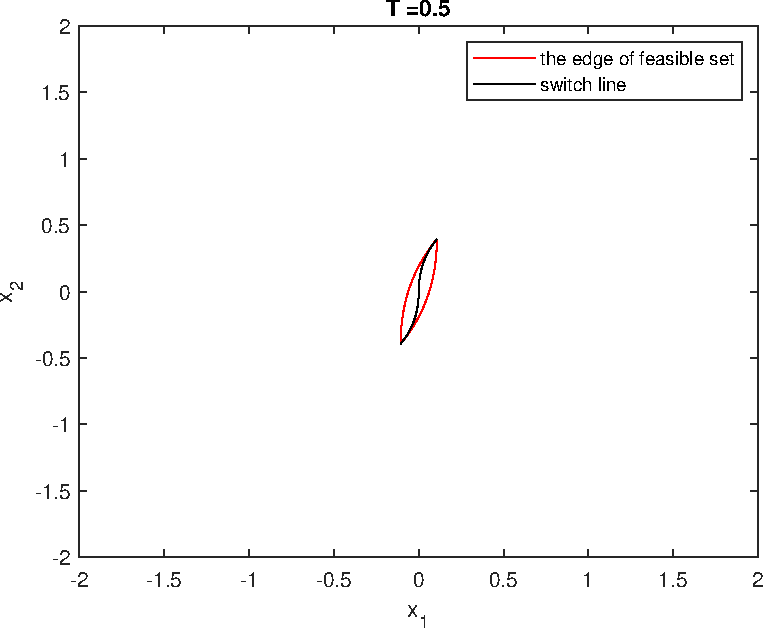
\includegraphics[width=7cm]{alpha_1_T_0.5.pdf} }}
    \qquad
    \subfloat {{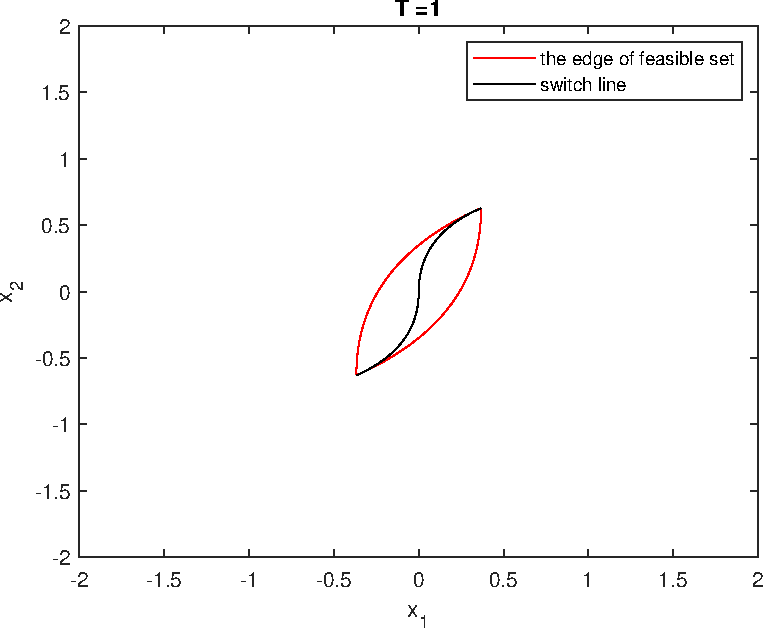
\includegraphics[width=7cm]{alpha_1_T_1.pdf} }}
    \\
    \subfloat {{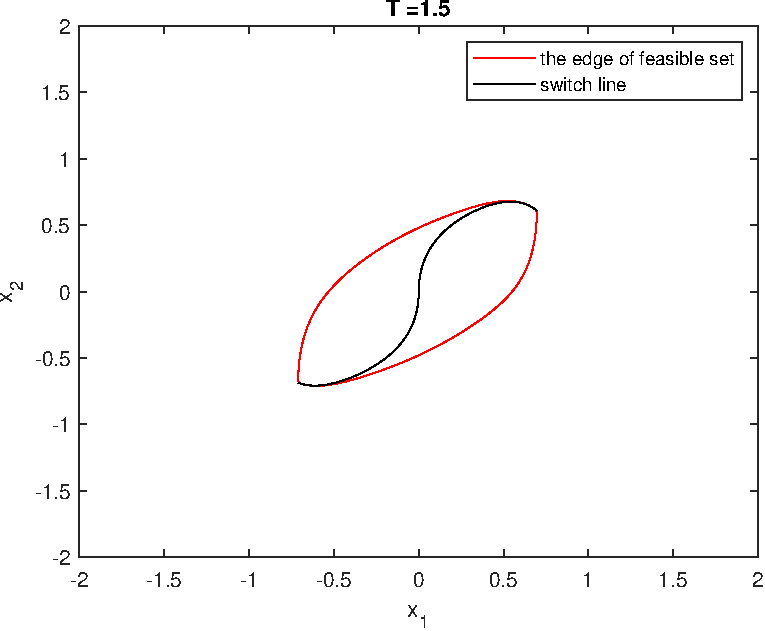
\includegraphics[width=7cm]{alpha_1_T_1.5.pdf} }}
    \qquad
    \subfloat {{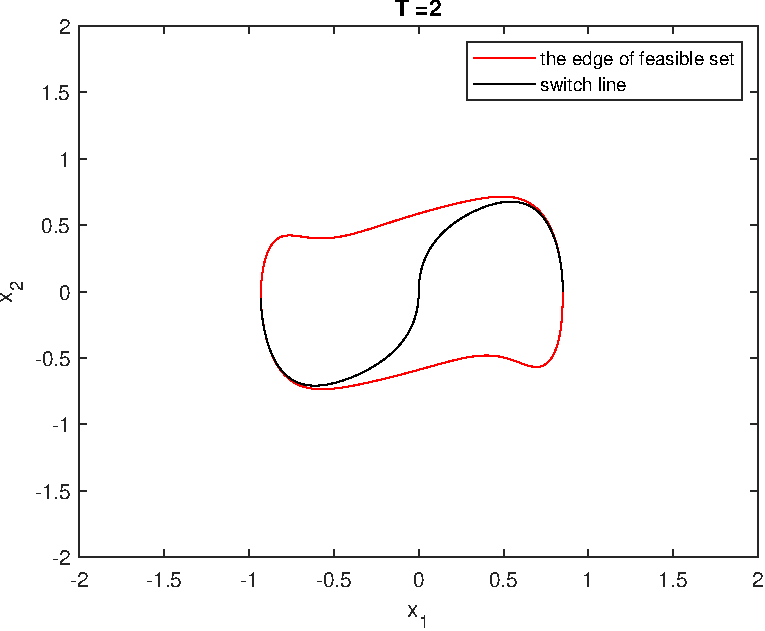
\includegraphics[width=7cm]{alpha_1_T_2.pdf} }}
\end{figure}
\newpage
\anonsubsection{Пример 2}
Данный пример иллюстрирет эволюцию множества достижимости при \( \alpha = 2 \). Видно, что при увеличении \( \alpha \) размеры множества достижимости увеличиваются. С течением времени оно, очевидно, также растет.
\begin{figure}[h]
    \centering
    \subfloat {{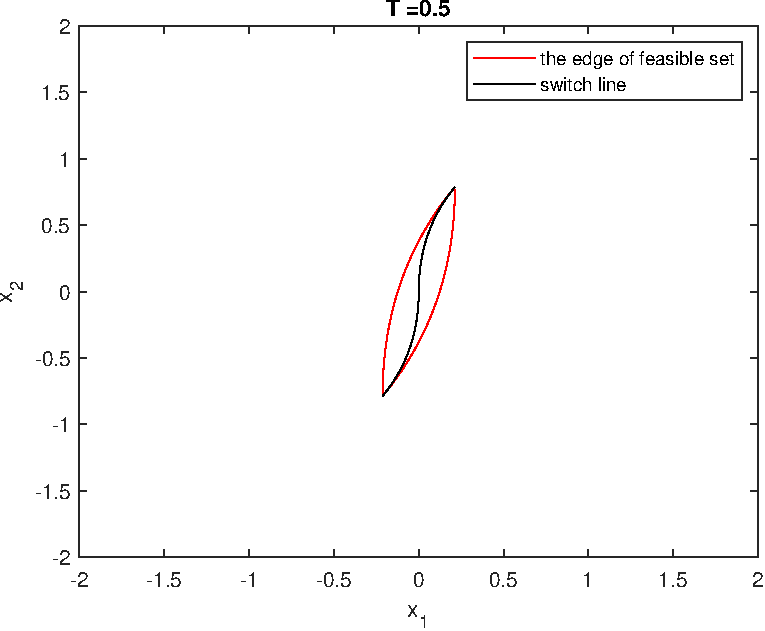
\includegraphics[width=7cm]{alpha_2_T_0.5.pdf} }}
    \qquad
    \subfloat {{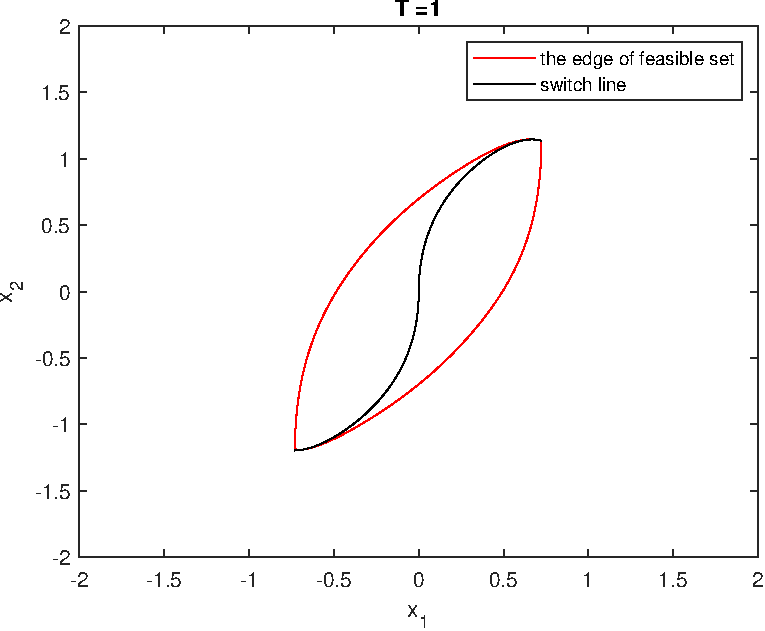
\includegraphics[width=7cm]{alpha_2_T_1.pdf} }}
    \\
    \subfloat {{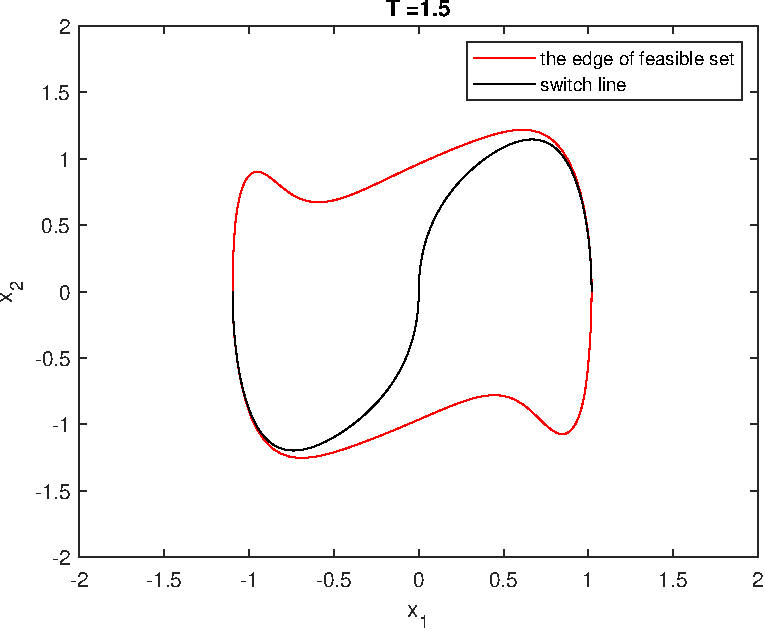
\includegraphics[width=7cm]{alpha_2_T_1.5.pdf} }}
    \qquad
    \subfloat {{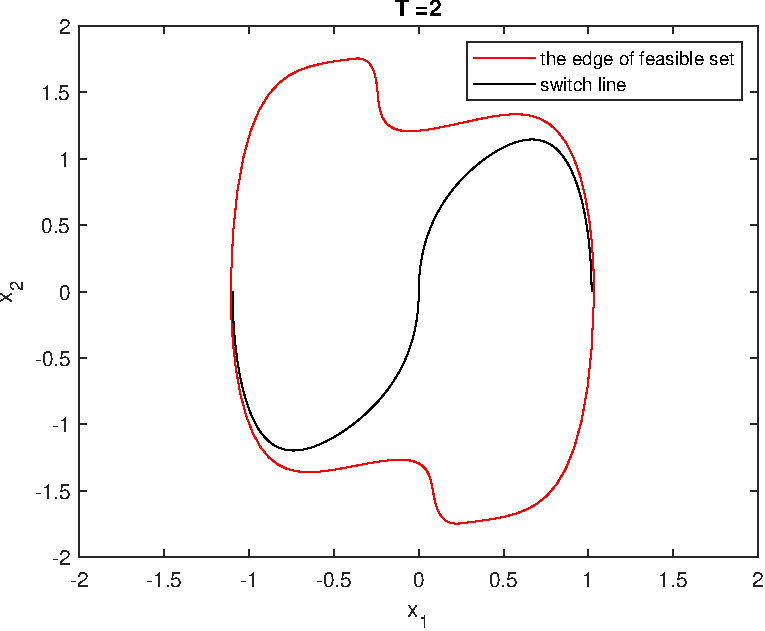
\includegraphics[width=7cm]{alpha_2_T_2.pdf} }}
\end{figure}
\newpage
\begin{thebibliography}{0}
\addcontentsline{toc}{section}{Список литературы}
\bibitem{1}
Ю.\,Н. Киселев, С.\,Н. Аввакумов, М.\,В. Орлов \emph{Оптимальное управление. Линейная теория и приложения:Учебное пособие} М.:МАКС Пресс, 2007
\bibitem{2}
Л.\,С. Понтрягин, В.\,Г. Болтянский , Р.\,В. Гамкрелидзе , Е.\,Ф. Мищенко \emph{Математическая теория оптимальных процессов} М.: Наука, 1983
\end{thebibliography}

\end{document}